\section{Perspectives}

\begin{frame}
\begin{block}{Perspectives du stage}
\begin{itemize}
    \item Obtenir un théorème de type Riesz–Fréchet–Kolmogorov
    \item Terminer la démonstration de la convergence
    \item Comprendre la dimension $\dim \mathcal{H}^\ensdiamantplat = 4 \, g$
    \item Réaliser des simulations numériques
\end{itemize}
\end{block}
\begin{block}{Cadre de la thèse}
\begin{itemize}
    \item Diffraction électromagnétique par un objet
    % \begin{figure}
    %     \centering
    %     \begin{tikzpicture}[
    scale=1.1,
    every node/.style={font=\footnotesize},
    every path/.append style={line cap=round}
]

\begin{scope}[shift={(0.5,0.25)}]
\draw[myblue, thick, ->] (-4,0) -- (-3,0);
\draw[myblue] (-3.7,-0.4) -- (-3.7,0.4);
\draw[myblue] (-3.5,-0.4) -- (-3.5,0.4) node[above] {onde incidente};
\draw[myblue] (-3.3,-0.4) -- (-3.3,0.4);
\end{scope}

\node[anchor=south west, inner sep=0] (obs) at (0,0) {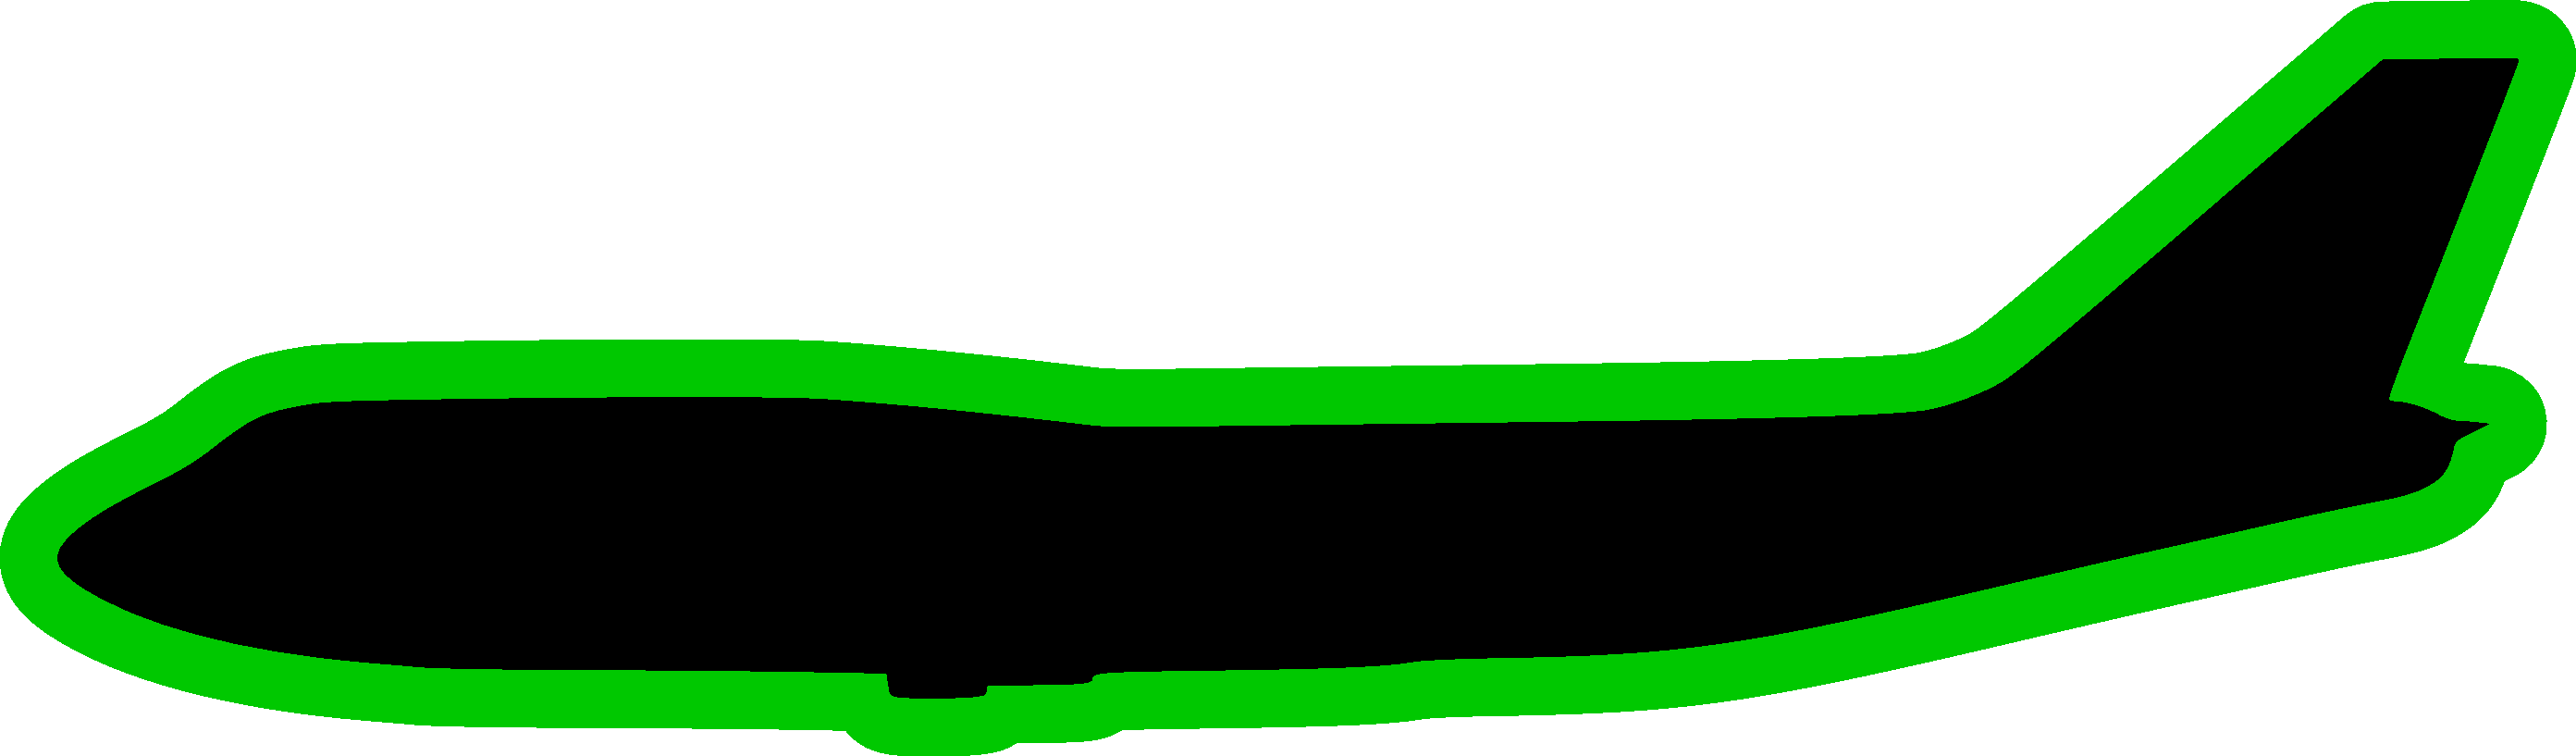
\includegraphics[width=2cm]{img/avion.pdf}};
\node[below=8pt] at (obs.center) {obstacle};
\node[mydarkgreen, right] at (obs.east) {$\Sigma$};

\begin{scope}[rotate=-45, shift={(0.03,0.25)}]
    \draw[decoration={expanding waves, segment length=3mm, angle=40}, decorate, myred] (0, 0) -- ++(-1.2,0) node[right=25pt] {onde diffractée};
    \draw[myred, thick, ->] (-0.2,0) -- (-1.3,0);
    \draw[myred, thick, ->, rotate around={-25:(0,0)}] (-0.2,0) -- (-1.3,0);
    \draw[myred, thick, ->, rotate around={25:(0,0)}] (-0.2,0) -- (-1.3,0);
\end{scope}

\end{tikzpicture}
    % \end{figure}
    \item Équations de Maxwell en régime harmonique
    \item Méthode des équations intégrales : \emph{Electric Field Integral Equation} sur {\color{mydarkgreen}$\surflisse$}
    \[
    \gamma^\mathrm{tan} \mathopen{}\left( \mathrm{i} \, \omega \mu_0 G \vec{J} + \frac{\mathrm{i}}{\omega \varepsilon_0} \grad G \, \mathrm{div} \vec{J} \right) = E^\mathrm{tan}_\mathrm{inc}
    % \gamma^\text{tan} T = \gamma^\text{tan} \left( \mathrm{i}\, \omega \mu_0 G + \frac{\mathrm{i}}{\omega \varepsilon_0} \grad G\, \text{div} \right)
    \]
    \item Matrices \textbf{pleines} et très \textbf{mal conditionnées} % $\implies$ méthodes très lentes
\end{itemize}
\begin{center}
\highlighttxt{\sftxt{Méthode de \textbf{préconditionnement} : identité de Calder\'on + $\text{div} (n \times \grad \varphi) = 0$}}
\end{center}
\begin{itemize}
    \item Malheureusement, cette identité ne passe pas bien au niveau discret
\end{itemize}
\end{block}
% \begin{exampleblock}{Enjeu principal de la thèse}
% \begin{itemize}
%     \item Proposer une méthodologie efficace et naturelle via la méthode \ddfv
% \end{itemize}
% \end{exampleblock}

\end{frame}